\section{Ejercicio 2}

Se pedía escribir un lote de tareas que simulara la utilización de una
computadora para resolver un problema de Data Mining y, simultáneamente, como
servidor para tres clientes que realizan tareas bloqueantes. Esto se realizó
utilizando una tarea \texttt{TaskCPU} con una duración de 500, y tres tareas de
tipo \texttt{TaskIORandom}. Esta tarea recibe tres parámetros ($ms\_cpu$, $bmin$
y $bmax$) y realiza, en tiempo $ms\_cpu$, una llamada bloqueante con una duración
aleatoria entre $bmin$ y $bmax$. En los tres casos se consideró $bmin = 1$ y
$bim = 4$, mientras que para $ms\_cpu$ se tomaron los valores $10$, $20$ y $30$.

A continuación se exponen los gráficos obtenidos, considerando un costo para el cambio de contexto de 5 ciclos de CPU.

\begin{figure}[H]
    \begin{center}
        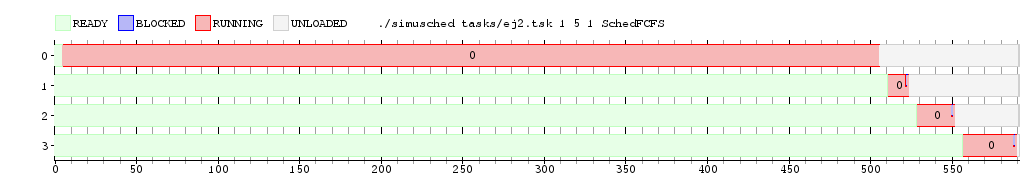
\includegraphics[width=1\columnwidth]{imagenes/ej2_1.png}
        \caption{Lote \texttt{ej2} corriendo en 1 núcleo}
    \end{center}
\end{figure}

\begin{figure}[H]
    \begin{center}
        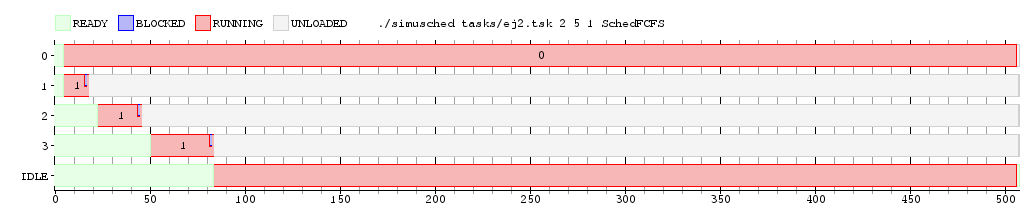
\includegraphics[width=1\columnwidth]{imagenes/ej2_2.png}
        \caption{Lote \texttt{ej2} corriendo en 2 núcleos}
    \end{center}
\end{figure}

\begin{figure}[H]
    \begin{center}
        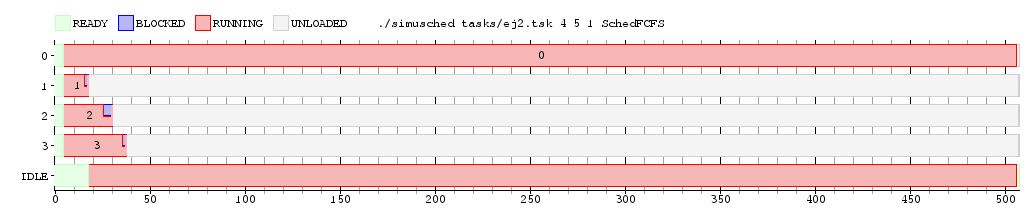
\includegraphics[width=1\columnwidth]{imagenes/ej2_3.png}
        \caption{Lote \texttt{ej2} corriendo en 4 núcleos}
    \end{center}
\end{figure}

Calculando, en los tres escenarios, la \emph{latencia} de cada tarea, se obtiene:

\begin{table}[H]
    \begin{center}
        \begin{tabular}{|c|c|c|c|c|}
            \hline
            & \multicolumn{4}{c|}{\textbf{Latencia}} \\ \hline
            \textbf{Cant. núcleos} & \texttt{TaskCPU} & \texttt{TaskIORandom (1)} & \texttt{TaskIORandom (2)} & \texttt{TaskIORandom (3)} \\ \hline
            1 & 5 & 511 & 531 & 561 \\
            2 & 5 & 5 & 24 & 53 \\
            4 & 5 & 5 & 5 & 5 \\ \hline
        \end{tabular}
    \end{center}
\end{table}

Teniendo en cuenta estos datos, resulta evidente que este modelo de
\emph{scheduling} resulta muy poco eficaz en un escenario como el planteado si
solo se cuenta con un único \emph{core}: la razón es que, al no contar con
desalojo, si el proceso que hace uso de la CPU durante 500 ciclos queda primero
en la cola del \emph{scheduler}, las demás tareas deberán esperar a que este
sea ejecutado en su totalidad para poder empezar a correr. Esto aumenta
excesivamente la \emph{latencia} de estos procesos. Los resultados obtenidos
con 2 núcleos son muy superiores, dado que todas las tareas cortas pueden
utilizar uno de los núcleos sin verse afectadas por el otro proceso extenso.
